\subsection{Characteristic as function of light intensity}

Based off of Table \ref{tab:variac_data} we are able to convert the values of our inputted lamp voltage and change it into intensity. We use these intensity values in relation with the current and voltage in Figure \ref{fig:intensity}.

In the voltage ramp seen in Figure \ref{fig:V_intensity} we are able to see that the voltage increases with more light, but the rate of voltage change is decreasing. This is due to a process known as thermalization, since some photons have more energy than the bandgap and this excess energy is put into the lattice rather than used for liberating atoms in the bandgap.

For the short circuited current, the intensity of the light is theorized to generate a linearly increasing amount of current as well. However a deviation from this idealization is seen in Figure \ref{fig:I_intensity}. The major issue that we will attribute this to is that the temperature of the panel increases as we go lower in intensity (due to previous runs) and this will decrease efficiency of the cell, leading to lower currents than are expected in our data. Generally we note that this non-ideal solar panel has a electron loss which does not scale with intensity, instead dominating at low intensities.

\begin{figure}[ht] 
  \begin{subfigure}[b]{0.45\linewidth}
    \centering
    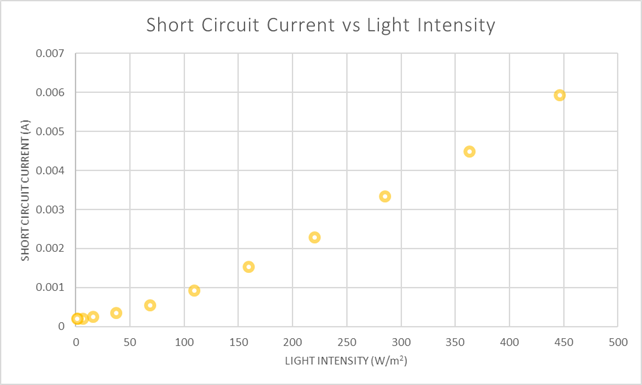
\includegraphics[width=0.90\linewidth]{figures/I_Intensity.png} 
    \caption{Short circuited current} 
    \label{fig:I_intensity} 
    \vspace{4ex}
  \end{subfigure}%% 
  \begin{subfigure}[b]{0.45\linewidth}
    \centering
    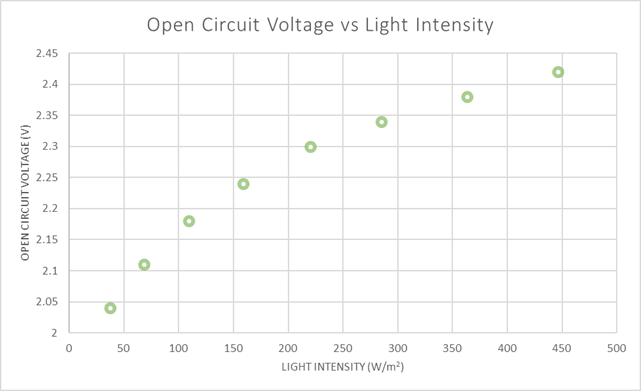
\includegraphics[width=0.90\linewidth]{figures/V_Intensity.png} 
    \caption{No Load Voltage} 
    \label{fig:V_intensity} 
    \vspace{4ex}
  \end{subfigure} 
  \caption{Solar cell current and voltage characteristics as a function of intensity ramps}
  \label{fig:intensity} 
\end{figure}

\clearpage

\subsection{Temperature Dependence of no-load voltage}

In Figure \ref{fig:temp} and Table \ref{tab:temp_effect_data} we see the data for the temperature relation of open circuit voltage. we first note that our data for low temperatures is noisy. This is likely due to inequal heating of the cell or due to the IR laser of the heat gun causing some generation of electrons which is inequal between different trials.

However we can see that as the temperature increases, the amount of voltage which is generated decreases. This is because voltage is the potential difference between the electrons at rest and those in an excited state. At colder temperatures that difference is lager then hotter temperatures. This is because when you are heating up the electron you are giving them energy so the hotter it gets the less the difference between the rest and excited states becomes.

\begin{figure}[h]
    \centering
    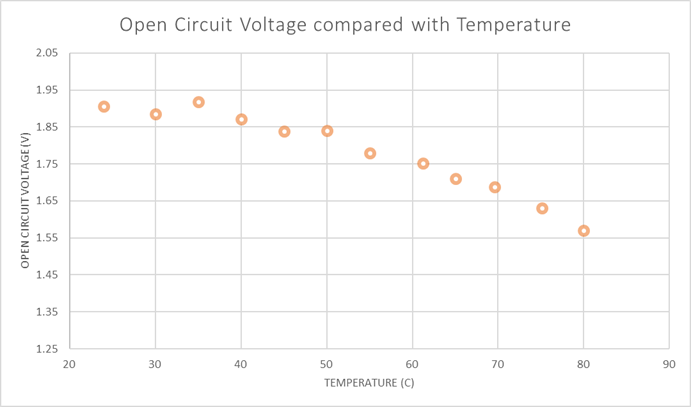
\includegraphics[width=.75\linewidth]{figures/temp.png}
    \caption{Voltage of the solar cell with an increasing temperature.}
    \label{fig:temp}
\end{figure}

\clearpage

\subsection{I-V characteristics of the solar cell}

\begin{figure}[ht] 
  \begin{subfigure}[b]{0.90\linewidth}
    \centering
    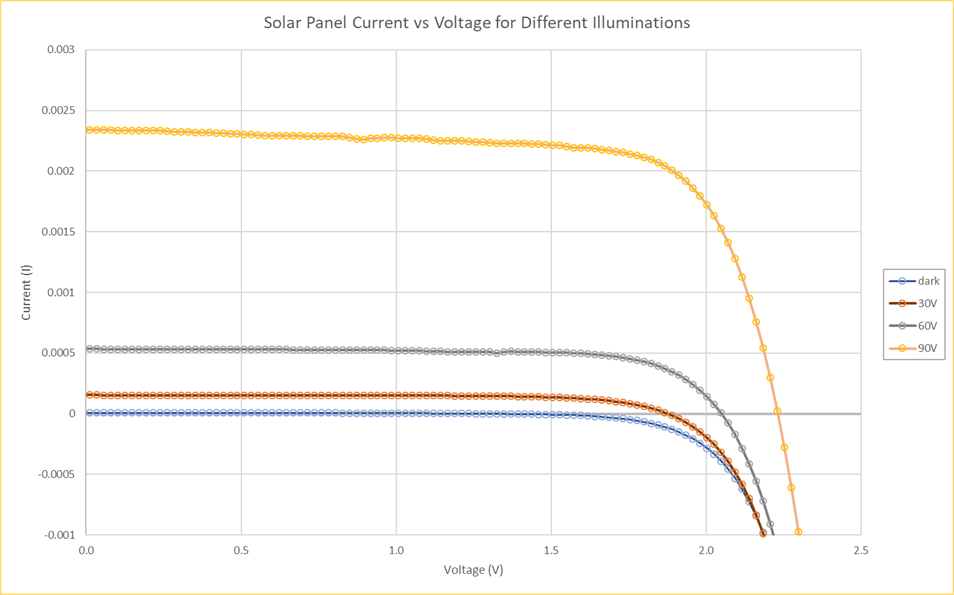
\includegraphics[width=0.90\linewidth]{figures/I_V_curves.png} 
    \caption{Current Voltage Curves} 
    \label{fig:I_V} 
    \vspace{4ex}
  \end{subfigure}\\%% 
  \begin{subfigure}[b]{0.90\linewidth}
    \centering
    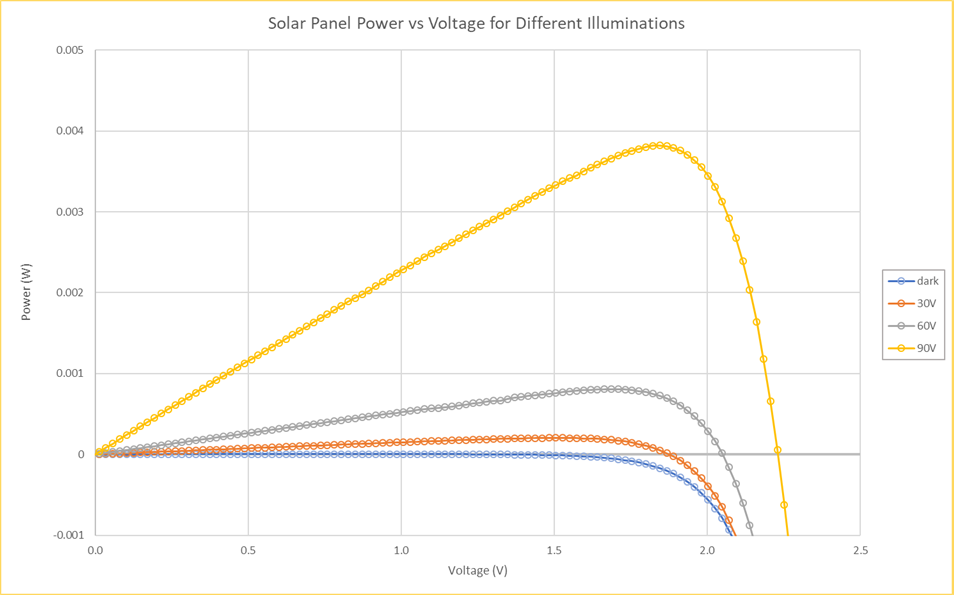
\includegraphics[width=0.90\linewidth]{figures/P_V_curves.png} 
    \caption{Power Voltage Curves} 
    \label{fig:P_V} 
    \vspace{4ex}
  \end{subfigure} 
  \caption{Voltage relationships for each of the four light intensities. These are varied and the values shown in Table \ref{tab:I_V} show the calculation of several quantities based off of these graphs}
  \label{fig:curves} 
\end{figure}

We see in Figure \ref{fig:I_V} that as more intense light is being inputted into the solar panel, the current dramatically increases. We see this in the dramatic changes between the dark to 30V and then successively for each of the increased intensities after that. The shape of the graph are as predicted from theory, however when compared to the ideally power generating solar cell we see that it is not very rectangular, indicating that the fill factor is not high. This is shown in our calculations shown in Table \ref{fig:I_V}. 

From Figure \ref{fig:P_V} we are able to see the power output of the cell as compared with the voltage. From this we are able to see that the maximal point is a sharp peak, meaning that if the cell is to be run optimally it will have to be run at a specific voltage. We also see the same relationship as seen in the Current vs Voltage graphs where the higher intensities scale with the higher currents/power.  

\begin{table}[ht]
    \centering
    \begin{tabular}{lllll}
                                   & \textbf{Dark} & \textbf{30 V} & \textbf{60 V} & \textbf{90V} \\ \hline
\textbf{$V_{oc}$ V}                & 1.256         & 1.867         & 2.048         & 2.229        \\
\textbf{$I_{sc}$ mA}               & 0.0062        & 0.154         & 0.534         & 2.34         \\
\textbf{$R_{sh}$ k$\Omega$}        & 30.62         & 0.452         & 0.136         & 0.048        \\
\textbf{$R_{s}$ k$\Omega$}         & 3853          & 288.5         & 57.8          & 24.48        \\ \hline
\textbf{Maximum Power (mW)}        & 0.0047        & 0.204         & 0.806         & 3.82         \\
\textbf{Current at Max Power (mW)} & 0.0054        & 0.204         & 0.478         & 2.07         \\
\textbf{Voltage at Max Power}      & 0.872         & 1.505         & 1.686         & 1.844        \\ \hline
\textbf{Fill Factor}               & 0.60          & 0.71          & 0.74          & 0.73         \\
\textbf{Maximum Efficiency}        & N/A           & 1.69\%        & 0.630\%       & 0.923\%      \\ \hline
\end{tabular}
    \caption{Quantities which are calculated based off of the data shown in Figure \ref{fig:curves}. }
    \label{tab:I_V}
\end{table}

\clearpage

\subsection{Carrier life time, response time }
 As mentioned in the lab manual the minority carrier life time for both the N silicon wafer sample and the P silicon wafer sample was measured to be between 10 mircoseconds and 20 mircro seconds. The reason that the carrier lifetime for the solar cell could be that a solar cell is made up of both n-type and p-type semiconductors.It is the flow of electrons through these two semiconductors that creates electricity. That means that both semiconductors have different recombination. Since the carrier lifetime is defined as the average time it takes for a minority carrier to recombine having two semiconductors with different minority carries with different recombination rates and the fact that the electrons are flowing would all lead to the longer minority carrier lifetime in a solar cell

